\documentclass{standalone}
\usepackage{tikz}
\usetikzlibrary{patterns, positioning}
\usepackage[sfdefault]{ClearSans} %% option 'sfdefault' activates Clear Sans as the default text font
\usepackage[T1]{fontenc}

\begin{document}
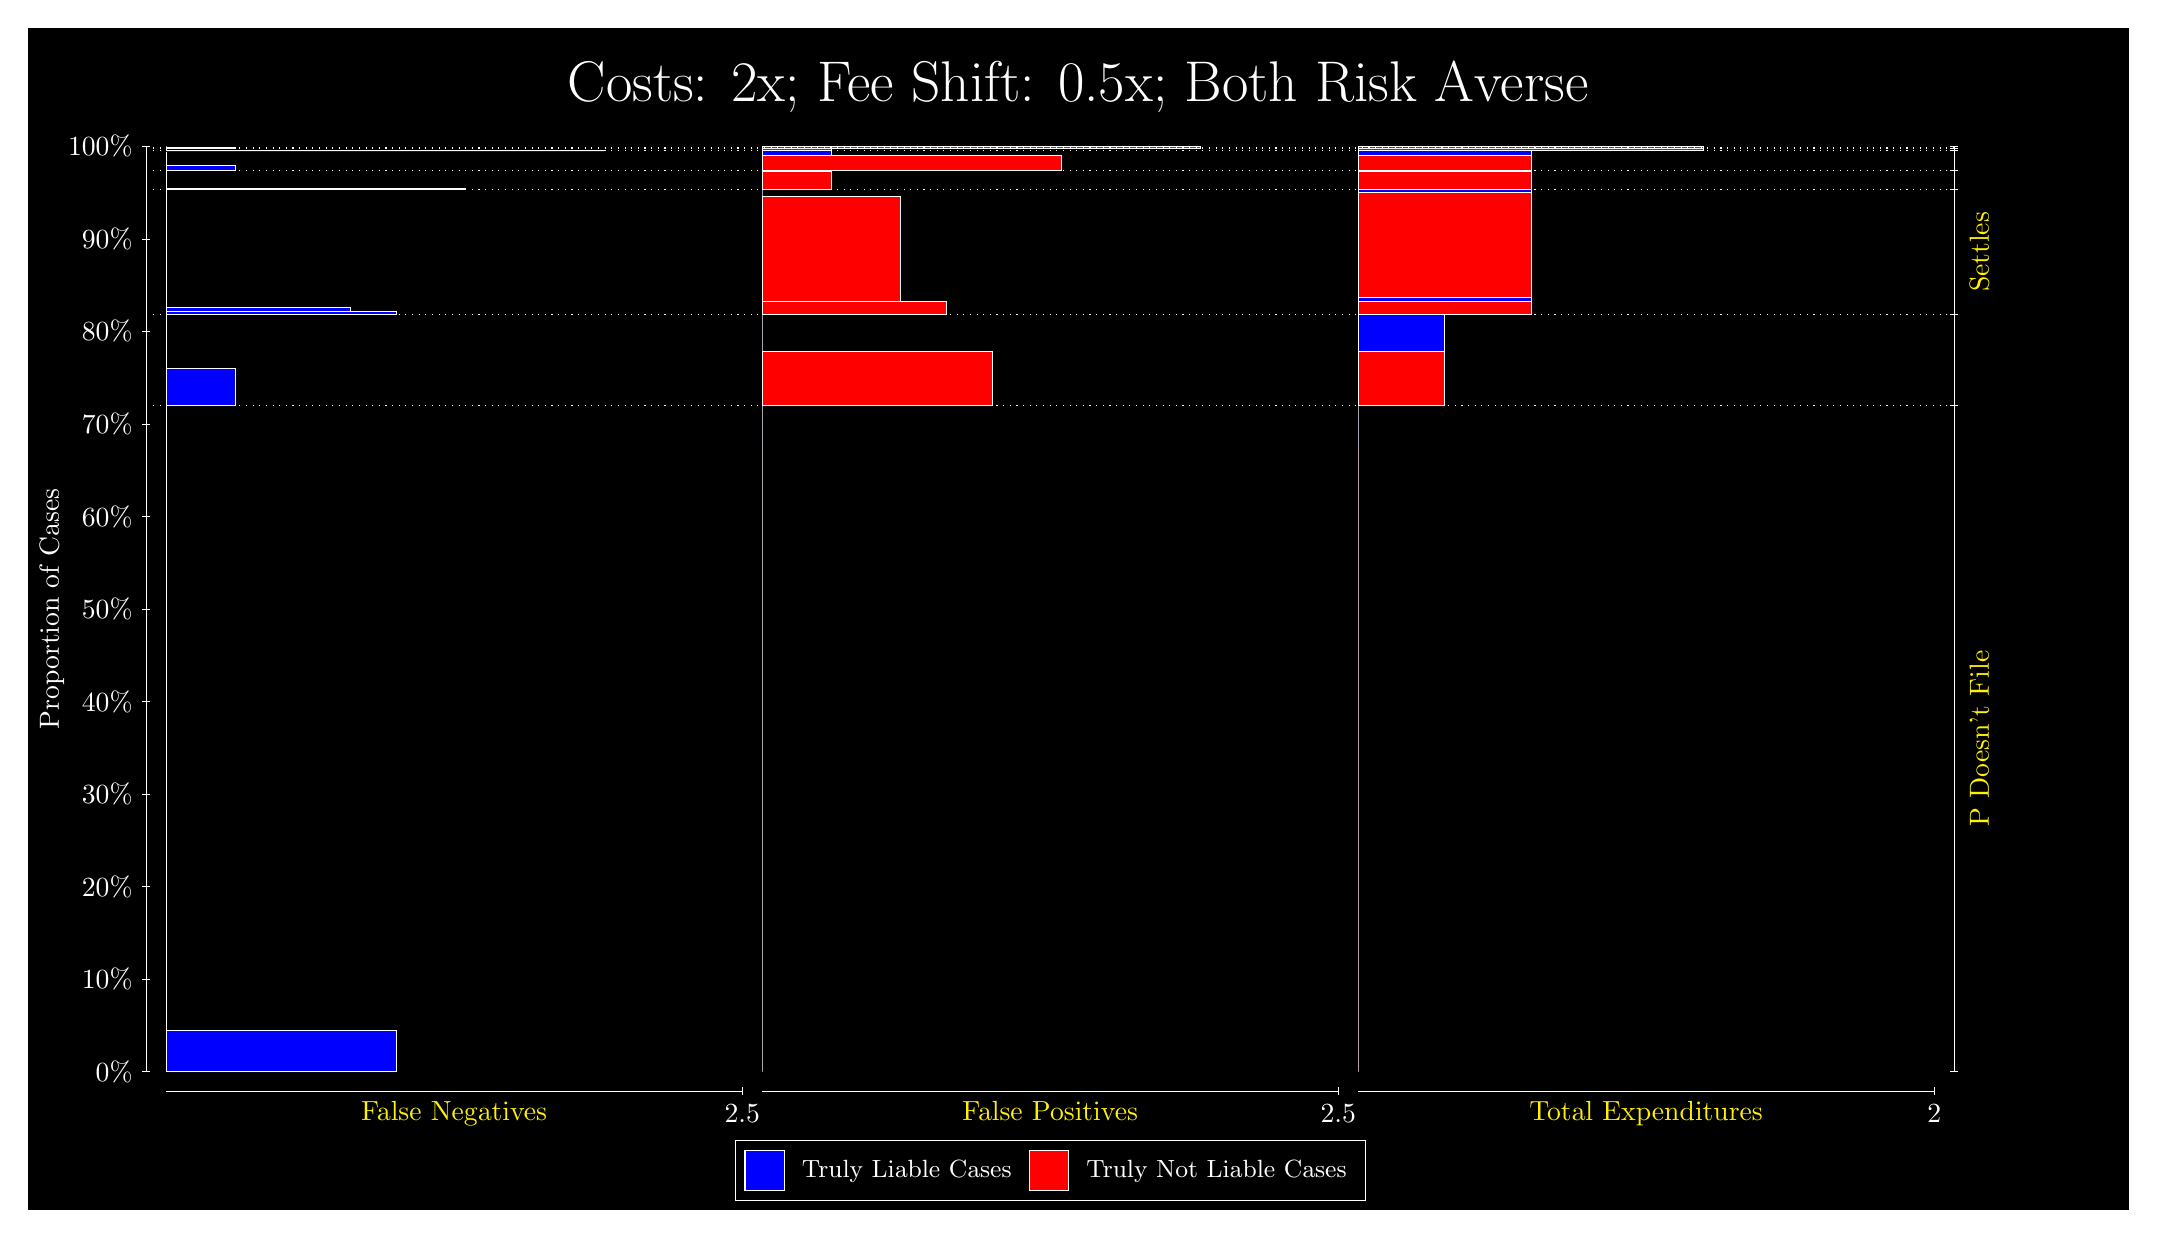
\begin{tikzpicture}
\draw[fill=black] (0,0) rectangle (26.667,15);
\draw[text=white] (0,13.5) rectangle (26.667,15) node[midway] {\huge Costs: 2x; Fee Shift: 0.5x; Both Risk Averse};
\draw[white, very thin] (1.5,1.75) -- (1.5,13.5);
\node[rotate=90, text=white, anchor=center] at (0.3, 7.625) {Proportion of Cases};
\draw[white, very thin] (1.45,1.75) -- (1.55,1.75);
\node[text=white, anchor=east] at (1.45, 1.75) {0\%};
\draw[white, very thin] (1.45,2.925) -- (1.55,2.925);
\node[text=white, anchor=east] at (1.45, 2.925) {10\%};
\draw[white, very thin] (1.45,4.1) -- (1.55,4.1);
\node[text=white, anchor=east] at (1.45, 4.1) {20\%};
\draw[white, very thin] (1.45,5.275) -- (1.55,5.275);
\node[text=white, anchor=east] at (1.45, 5.275) {30\%};
\draw[white, very thin] (1.45,6.45) -- (1.55,6.45);
\node[text=white, anchor=east] at (1.45, 6.45) {40\%};
\draw[white, very thin] (1.45,7.625) -- (1.55,7.625);
\node[text=white, anchor=east] at (1.45, 7.625) {50\%};
\draw[white, very thin] (1.45,8.8) -- (1.55,8.8);
\node[text=white, anchor=east] at (1.45, 8.8) {60\%};
\draw[white, very thin] (1.45,9.975) -- (1.55,9.975);
\node[text=white, anchor=east] at (1.45, 9.975) {70\%};
\draw[white, very thin] (1.45,11.15) -- (1.55,11.15);
\node[text=white, anchor=east] at (1.45, 11.15) {80\%};
\draw[white, very thin] (1.45,12.325) -- (1.55,12.325);
\node[text=white, anchor=east] at (1.45, 12.325) {90\%};
\draw[white, very thin] (1.45,13.5) -- (1.55,13.5);
\node[text=white, anchor=east] at (1.45, 13.5) {100\%};

\draw[white, very thin] (24.457,1.75) -- (24.457,13.5);
\draw[white, very thin] (24.407,1.75) -- (24.507,1.75);
\node[anchor=west] at (24.407, 1.75) {};
\draw[white, very thin] (24.407,10.209) -- (24.507,10.209);
\node[anchor=west] at (24.407, 10.209) {};
\draw[white, very thin] (24.407,11.365) -- (24.507,11.365);
\node[anchor=west] at (24.407, 11.365) {};
\draw[white, very thin] (24.407,12.954) -- (24.507,12.954);
\node[anchor=west] at (24.407, 12.954) {};
\draw[white, very thin] (24.407,13.195) -- (24.507,13.195);
\node[anchor=west] at (24.407, 13.195) {};
\draw[white, very thin] (24.407,13.444) -- (24.507,13.444);
\node[anchor=west] at (24.407, 13.444) {};
\draw[white, very thin] (24.407,13.479) -- (24.507,13.479);
\node[anchor=west] at (24.407, 13.479) {};
\draw[white, very thin] (24.407,13.5) -- (24.507,13.5);
\node[anchor=west] at (24.407, 13.5) {};

\draw[white, very thin, fill=blue] (1.75,1.75) rectangle (4.6775,2.2801);
\draw[white, very thin, fill=red] (1.75,2.2801) rectangle (1.75,10.209);
\draw[white, very thin, fill=blue] (1.75,10.209) rectangle (2.6283,10.678);
\draw[white, very thin, fill=red] (1.75,10.678) rectangle (1.75,11.365);
\draw[white, very thin, fill=blue] (1.75,11.365) rectangle (4.6775,11.408);
\draw[white, very thin, fill=blue] (1.75,11.408) rectangle (4.092,11.46);
\draw[white, very thin, fill=red] (1.75,11.46) rectangle (1.75,12.954);
\draw[white, very thin, fill=blue] (1.75,12.954) rectangle (5.5558,12.971);
\draw[white, very thin, fill=red] (1.75,12.971) rectangle (1.75,13.195);
\draw[white, very thin, fill=blue] (1.75,13.195) rectangle (2.6283,13.254);
\draw[white, very thin, fill=red] (1.75,13.254) rectangle (1.75,13.444);
\draw[white, very thin, fill=blue] (1.75,13.444) rectangle (7.3123,13.446);
\draw[white, very thin, fill=red] (1.75,13.446) rectangle (1.75,13.479);
\draw[white, very thin, fill=blue] (1.75,13.479) rectangle (2.6283,13.483);
\draw[white, very thin, fill=red] (1.75,13.483) rectangle (1.75,13.5);
\draw[white, very thin, fill=red] (9.3189,1.75) rectangle (9.3189,9.6786);
\draw[white, very thin, fill=blue] (9.3189,9.6786) rectangle (9.3189,10.209);
\draw[white, very thin, fill=red] (9.3189,10.209) rectangle (12.246,10.896);
\draw[white, very thin, fill=blue] (9.3189,10.896) rectangle (9.3189,11.365);
\draw[white, very thin, fill=red] (9.3189,11.365) rectangle (11.661,11.531);
\draw[white, very thin, fill=red] (9.3189,11.531) rectangle (11.075,12.86);
\draw[white, very thin, fill=blue] (9.3189,12.86) rectangle (9.3189,12.954);
\draw[white, very thin, fill=red] (9.3189,12.954) rectangle (10.197,13.178);
\draw[white, very thin, fill=blue] (9.3189,13.178) rectangle (9.3189,13.195);
\draw[white, very thin, fill=red] (9.3189,13.195) rectangle (13.125,13.385);
\draw[white, very thin, fill=blue] (9.3189,13.385) rectangle (10.197,13.444);
\draw[white, very thin, fill=red] (9.3189,13.444) rectangle (10.197,13.477);
\draw[white, very thin, fill=blue] (9.3189,13.477) rectangle (9.3189,13.479);
\draw[white, very thin, fill=red] (9.3189,13.479) rectangle (14.881,13.496);
\draw[white, very thin, fill=blue] (9.3189,13.496) rectangle (11.954,13.5);
\draw[white, very thin, fill=red] (16.888,1.75) rectangle (16.888,9.6786);
\draw[white, very thin, fill=blue] (16.888,9.6786) rectangle (16.888,10.209);
\draw[white, very thin, fill=red] (16.888,10.209) rectangle (17.986,10.896);
\draw[white, very thin, fill=blue] (16.888,10.896) rectangle (17.986,11.365);
\draw[white, very thin, fill=red] (16.888,11.365) rectangle (19.083,11.531);
\draw[white, very thin, fill=blue] (16.888,11.531) rectangle (19.083,11.583);
\draw[white, very thin, fill=red] (16.888,11.583) rectangle (19.083,12.912);
\draw[white, very thin, fill=blue] (16.888,12.912) rectangle (19.083,12.954);
\draw[white, very thin, fill=red] (16.888,12.954) rectangle (19.083,13.178);
\draw[white, very thin, fill=blue] (16.888,13.178) rectangle (19.083,13.195);
\draw[white, very thin, fill=red] (16.888,13.195) rectangle (19.083,13.385);
\draw[white, very thin, fill=blue] (16.888,13.385) rectangle (19.083,13.444);
\draw[white, very thin, fill=red] (16.888,13.444) rectangle (21.279,13.477);
\draw[white, very thin, fill=blue] (16.888,13.477) rectangle (21.279,13.479);
\draw[white, very thin, fill=red] (16.888,13.479) rectangle (21.279,13.496);
\draw[white, very thin, fill=blue] (16.888,13.496) rectangle (21.279,13.5);
\draw[white, dotted] (1.5,10.209) -- (24.457,10.209);
\draw[white, dotted] (1.5,11.365) -- (24.457,11.365);
\draw[white, dotted] (1.5,12.954) -- (24.457,12.954);
\draw[white, dotted] (1.5,13.195) -- (24.457,13.195);
\draw[white, dotted] (1.5,13.444) -- (24.457,13.444);
\draw[white, dotted] (1.5,13.479) -- (24.457,13.479);
\draw[white, very thin] (1.75,1.5) -- (9.0689,1.5);
\node[text=yellow, anchor=north] at (5.4094, 1.5) {False Negatives};
\draw[white, very thin] (9.0689,1.45) -- (9.0689,1.55);
\node[text=white, anchor=north] at (9.0689, 1.45) {2.5};

\draw[white, very thin] (9.3189,1.5) -- (16.638,1.5);
\node[text=yellow, anchor=north] at (12.978, 1.5) {False Positives};
\draw[white, very thin] (16.638,1.45) -- (16.638,1.55);
\node[text=white, anchor=north] at (16.638, 1.45) {2.5};

\draw[white, very thin] (16.888,1.5) -- (24.207,1.5);
\node[text=yellow, anchor=north] at (20.547, 1.5) {Total Expenditures};
\draw[white, very thin] (24.207,1.45) -- (24.207,1.55);
\node[text=white, anchor=north] at (24.207, 1.45) {2};

\node[text=yellow, centered, rotate=90] at (24.777, 5.9794) {P Doesn't File};

\node[text=yellow, centered, rotate=90] at (24.777, 12.16) {Settles};





\draw (12.978300999999998,1.5) node[draw=none] (baseCoordinate) {};
\begin{scope}[align=center]
        \matrix[scale=0.5, draw=white, below=0.5cm of baseCoordinate, nodes={draw}, column sep=0.1cm]{
            \node[rectangle, draw, minimum width=0.5cm, minimum height=0.5cm, fill=blue] {}; &
            \node[draw=none, font=\small, text=white] (B) {Truly Liable Cases}; &
            \node[rectangle, draw, minimum width=0.5cm, minimum height=0.5cm, fill=red] {}; &
            \node[draw=none, font=\small, text=white] (B) {Truly Not Liable Cases}; \\
            };
\end{scope}

\end{tikzpicture}
\end{document}